% Results and discussion (journal format, 2026-11-19). Numbers from paper/tables/* (scripts/build_paper.py),
% results/stats/e5_convergence.*, results/stats/e7_montecarlo.*, scripts/paper_figures.py; supplement items via \Sref.
\section{Results and discussion}
\label{sec:results}

\subsection{Overall comparison}
Table~\ref{tab:summary} summarises both suites. On Suite A, \ours{} has the best IGD and HV on all 12 instances, with a
mean IGD 62\% below IMOEA/D's, the strongest baseline, and the first Friedman rank on both metrics. On Suite B it is
better than IMOEA/D on 43 of 45 instances in IGD and on 42 in HV. IMEA-IED, IP-MOEA, NSGA-III, the Jin backbone and
IMOEA-DQN lose on every instance, and IMOEA/D-AWN is never better. NSGA-II reaches a lower IGD on 4--5 instances, all
100-task workflows with data $\times 1$, where the search space is small enough for plain non-dominated sorting to
converge, but never a higher HV. Per-instance results are in Tables~\Sref{tab:suitea_igd}--\Sref{tab:suiteb_hv_jin} of
the supplementary material, and the list-scheduling heuristics are 16--33 times worse in IGD than \ours{}
(Table~\Sref{tab:heuristics}).

% generated by scripts/build_paper.py; do not edit by hand
\begin{table*}[!htbp]
\centering
\footnotesize
\caption{Results on both suites: mean IGD ($\times10^{-2}$) and HV over instances, the number of instances on which each method is significantly better / worse / not different from \ours{} (Wilcoxon rank-sum, Holm-corrected, $\alpha = 0.05$), the mean Vargha--Delaney $A_{12}$ by IGD (probability that a run of \ours{} has the lower IGD), and the mean Friedman rank by IGD (Nemenyi critical difference 3.91 on Suite A, 2.02 on Suite B). Per-instance results are in the supplementary material.}
\label{tab:summary}
\setlength{\tabcolsep}{3pt}
\begin{tabular}{lcccccccccccc}
\toprule
& \multicolumn{6}{c}{Suite A (12 instances)} & \multicolumn{6}{c}{Suite B (45 instances)} \\
\cmidrule(lr){2-7}\cmidrule(lr){8-13}
Method & IGD & HV & IGD $+/-/\approx$ & HV $+/-/\approx$ & $A_{12}$ & Rank & IGD & HV & IGD $+/-/\approx$ & HV $+/-/\approx$ & $A_{12}$ & Rank \\
\midrule
\ours{} & \textbf{1.22} & \textbf{0.819} & -- & -- & -- & 1.00 & \textbf{1.86} & \textbf{0.949} & -- & -- & -- & 1.29 \\
IMOEA/D & 3.19 & 0.797 & 0/12/0 & 0/12/0 & 1.00 & 2.83 & 2.57 & 0.935 & 1/43/1 & 2/42/1 & 0.92 & 2.69 \\
IMOEA/D-AWN & 2.91 & 0.797 & 0/12/0 & 0/12/0 & 1.00 & 2.42 & 4.44 & 0.915 & 0/43/2 & 0/44/1 & 0.95 & 3.29 \\
IMEA-IED & 12.40 & 0.691 & 0/12/0 & 0/12/0 & 1.00 & 7.17 & 13.34 & 0.828 & 0/45/0 & 0/45/0 & 1.00 & 7.73 \\
IP-MOEA & 14.71 & 0.658 & 0/12/0 & 0/12/0 & 1.00 & 8.50 & 12.24 & 0.822 & 0/45/0 & 0/45/0 & 1.00 & 6.98 \\
NSGA-II (mid) & 4.84 & 0.770 & 0/12/0 & 0/12/0 & 1.00 & 4.50 & 6.51 & 0.882 & 4/40/1 & 0/44/1 & 0.90 & 3.82 \\
NSGA-II (int) & 4.80 & 0.771 & 0/12/0 & 0/12/0 & 1.00 & 4.25 & 6.57 & 0.882 & 5/40/0 & 0/44/1 & 0.89 & 4.09 \\
NSGA-III & 13.61 & 0.690 & 0/12/0 & 0/12/0 & 1.00 & 7.75 & 15.42 & 0.822 & 0/45/0 & 0/45/0 & 1.00 & 8.40 \\
IMOEA-DQN (fixed) & 11.66 & 0.635 & 0/12/0 & 0/12/0 & 1.00 & 6.67 & 11.64 & 0.805 & 0/45/0 & 0/45/0 & 1.00 & 6.78 \\
IMOEA-DQN & 25.43 & 0.605 & 0/12/0 & 0/12/0 & 1.00 & 9.92 & 22.94 & 0.736 & 0/45/0 & 0/45/0 & 1.00 & 9.93 \\
\bottomrule
\end{tabular}
\end{table*}


The Jin backbone, which differs from \ours{} only in Rank C and the mating, has a six times higher mean IGD on Suite B
(0.116 against 0.019), and its gap grows with the size of the DAG, from 0.052 at 100 tasks to 0.175 at 1000, as the stall
analysis of Section~\ref{sec:stall} predicts. The published IMOEA-DQN is last on both suites; its learned controller
makes it worse than its own backbone with a fixed action, which Section~\ref{sec:learned} explains.

The predicted intervals of \ours{} are slightly wider than IMOEA/D's (Suite B imprecision 60.9 against 57.8;
Table~\Sref{tab:suiteb_imprecision}). \ours{} spends no selection places on the uncertainty tier ($\gamma = 0$); on the
training instances, an uncertainty share of $\gamma = 1/6$ narrows the intervals by 10\% at a small cost in IGD
(Fig.~\Sref{fig:a3_tradeoff}), so a user who values predictable performance can trade some convergence for precision.
The methods with the narrowest intervals, IMOEA-DQN and the heuristics, owe them to very small fronts.

\subsection{Statistical significance}
Fig.~\ref{fig:cd} places the mean Friedman ranks of all methods on Suite B. On IGD, \ours{} (rank 1.29) is significantly
better than every method except IMOEA/D and IMOEA/D-AWN, whose ranks lie within the critical difference of 2.02; on HV
the same holds, with \ours{} at rank 1.09. The per-instance Wilcoxon tests (Table~\ref{tab:summary}) separate \ours{}
from these two as well: IMOEA/D is significantly worse on 43 of 45 instances in IGD and IMOEA/D-AWN on 43. With 12
instances, the critical difference on Suite A is 3.91 ranks, so there the per-instance tests carry the evidence.

\begin{figure}[pos=htbp]
\centering
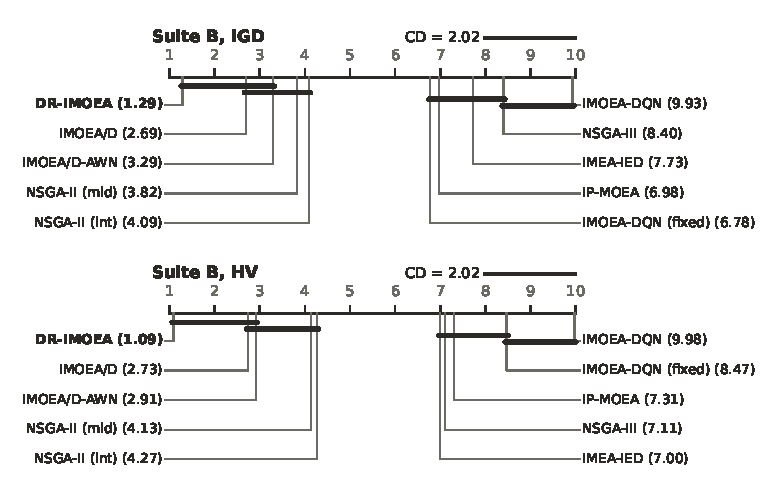
\includegraphics[width=\columnwidth]{figures/cd_diagram.pdf}
\caption{Critical-difference diagrams of the mean Friedman ranks on the 45 Suite B instances (Nemenyi test,
$\alpha = 0.05$). Methods joined by a bar are not significantly different.}
\label{fig:cd}
\end{figure}

The comparison with IMOEA/D depends on the normalisation at one size only. Repeating it with four different method
pools defining the normalisation and the reference front (Table~\Sref{tab:robustness}) leaves every verdict on Suite A
and up to 400 tasks, and every HV verdict, unchanged. At 1000 tasks, however, IMOEA/D has the lower IGD on 6--9 of the
15 instances when only the strong methods form the pool, so we read the 1000-task results on HV, where \ours{} is better
on 12 of 15.

\subsection{Pareto front analysis}
\label{sec:fronts}
The final fronts in Fig.~\ref{fig:fronts} compare \ours{} with three other methods on a Suite A and a large Suite B
instance, using for each method the run with the median IGD. On medium-250, \ours{}'s front reaches a lower cost than
the other fronts at almost every makespan and extends much further towards slow, cheap schedules, which the other
methods barely reach; in the makespan--energy projection the fronts lie close together, \ours{} trading slightly more
energy for its lower cost, which is a trade-off within the three-objective front rather than dominance. On
cybershake-1000, the fronts of \ours{} and IMOEA/D overlap closely in their middle part, where \ours{}'s solutions dominate
most of IMOEA/D's, while IMOEA/D reaches further to the cheapest schedules.

\begin{figure*}[pos=tbp]
\centering
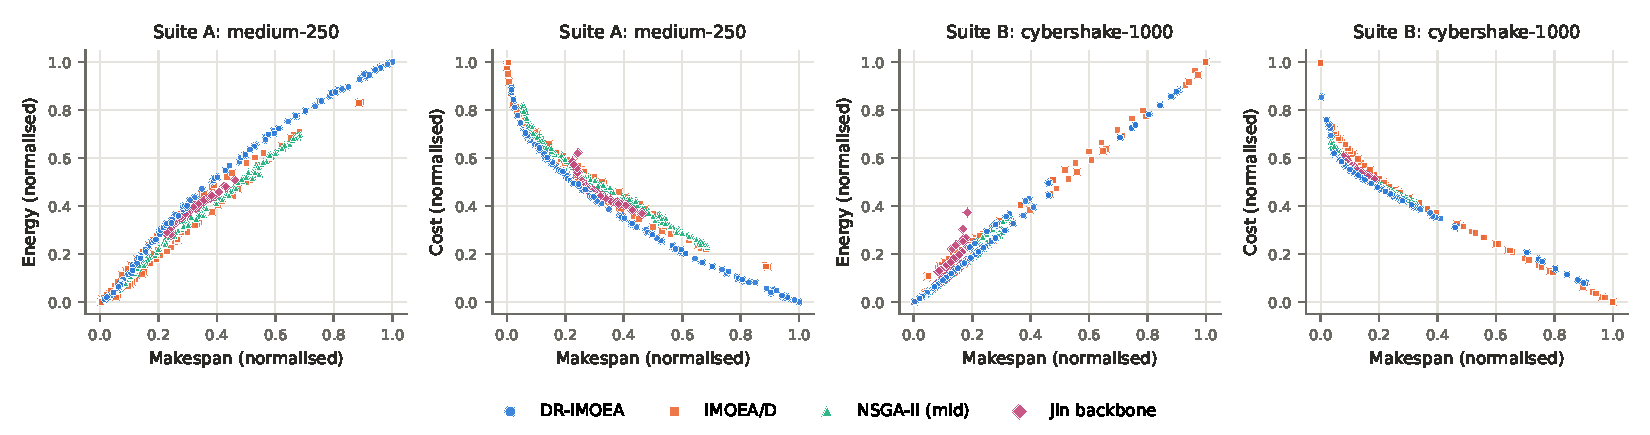
\includegraphics[width=\textwidth]{figures/fronts.pdf}
\caption{Final fronts (interval midpoints, normalised) of four methods, projected onto makespan--energy and
makespan--cost, on a Suite A and a Suite B instance with data $\times 20$; for each method the run with the median IGD.}
\label{fig:fronts}
\end{figure*}

For a decision maker the two methods therefore offer different parts of the trade-off on very large workflows. For most
schedules IMOEA/D finds, \ours{} offers one that is at least as good in all three objectives. IMOEA/D additionally
covers the cheapest schedules, which keep more tasks on the devices, where computation costs nothing, at the price of a
longer makespan or more device energy. When cost is the overriding criterion, the cost end of IMOEA/D's front is worth
consulting; otherwise \ours{}'s front is the better choice, and since both are computed at a similar cost
(Section~\ref{sec:runtime}) the two fronts can simply be merged.

\subsection{Convergence}
\label{sec:convergence}
Fig.~\ref{fig:e5_convergence} plots IGD and HV against the generation. On medium-250, \ours{} pulls ahead of every method
by generation 100 and ends with a third of IMOEA/D's IGD (0.012 against 0.035). On montage-400, IMOEA/D converges faster
at first and \ours{} overtakes it at about generation 350. On the 1000-task workflows the two are close throughout,
\ours{} ends slightly ahead, and both curves are still falling at generation 1000, so at this size the budget, not the
method, limits the result. The other methods stall far above. IMOEA-DQN starts worse than the initial population
because its early actions concentrate the search in one region.

\begin{figure*}[pos=tbp]
\centering
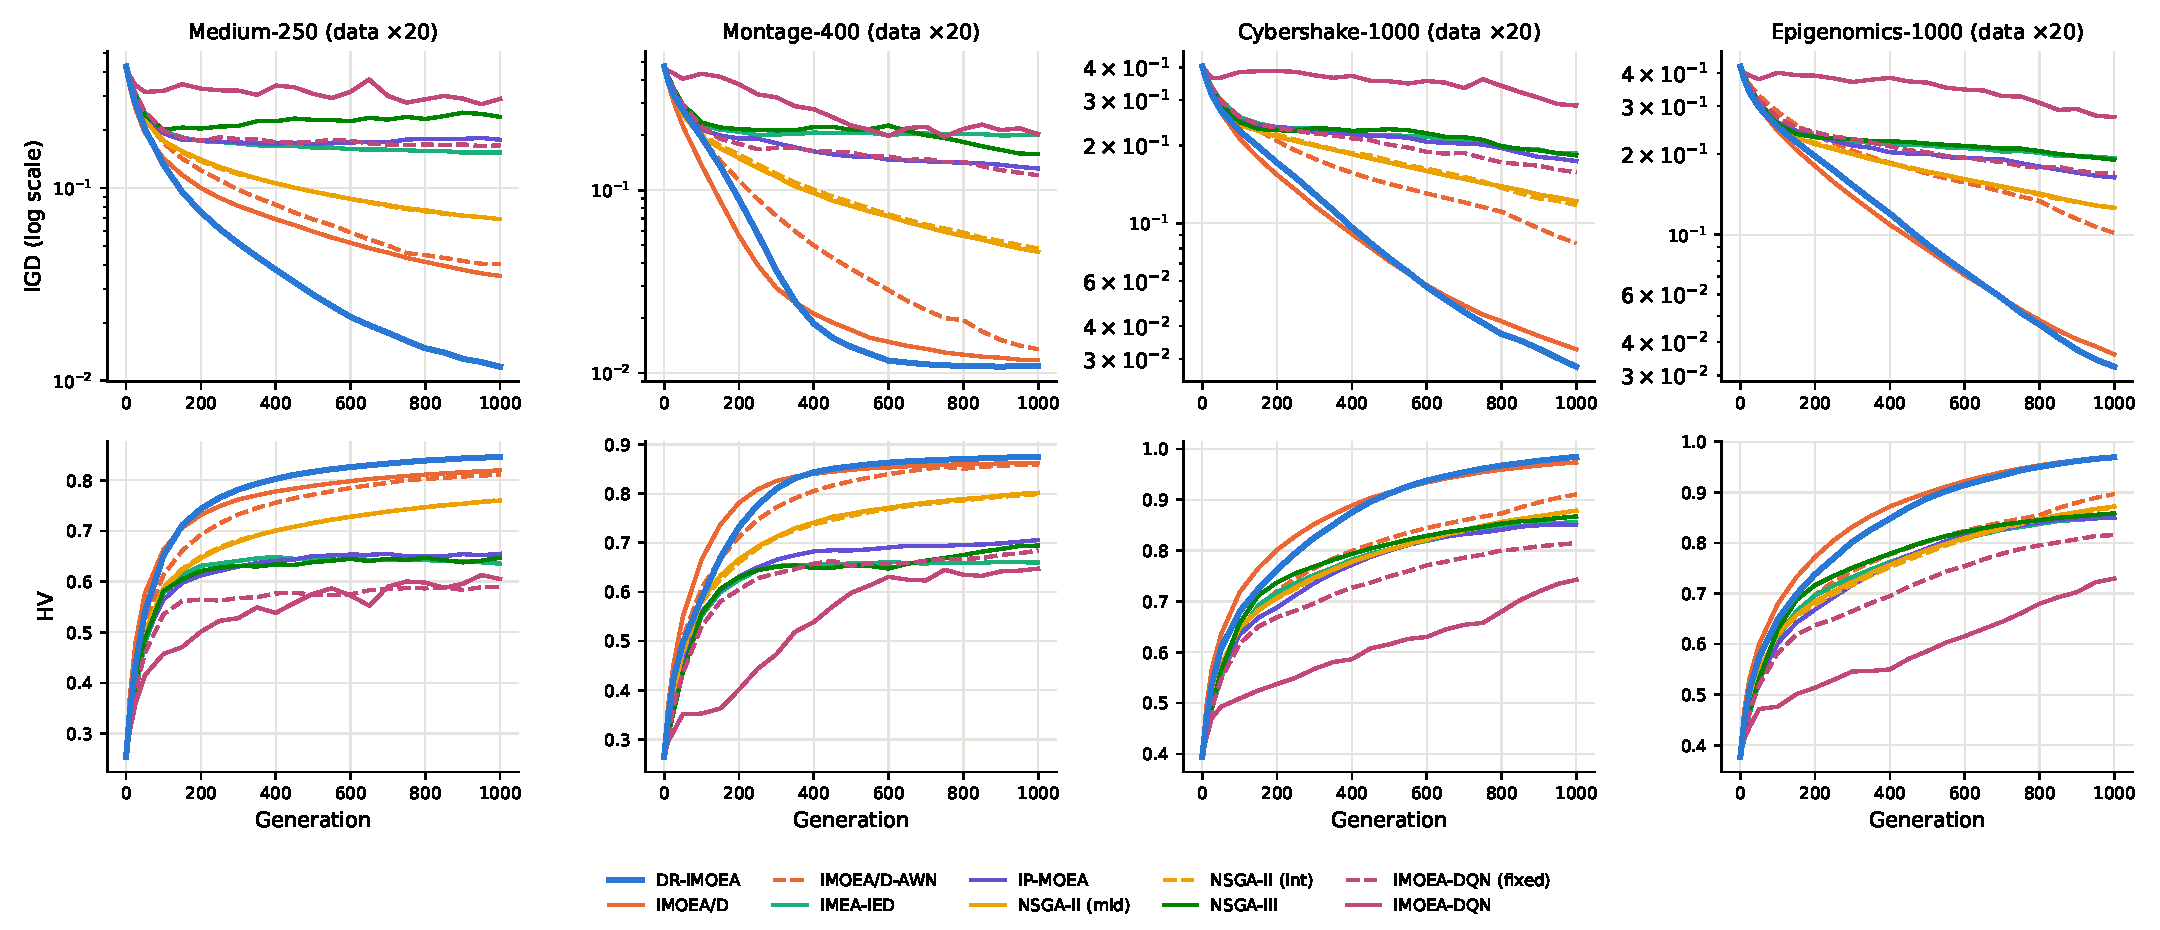
\includegraphics[width=\textwidth]{figures/e5_convergence.pdf}
\caption{Mean IGD (top, log scale) and HV (bottom) against the generation, 10 runs per method, on one Suite A and three
Suite B instances (data $\times 20$).}
\label{fig:e5_convergence}
\end{figure*}

\subsection{Ablation study}
\label{sec:ablation}
Table~\ref{tab:ablation} builds \ours{} from the Jin backbone on the 12 Suite A instances. The Tchebycheff Rank C halves
the mean IGD (0.119 to 0.058), the ICD tie-break lowers it to 0.048, and neighbourhood mating brings it to 0.0135; the
tuned mating parameters reach 0.0102. The rank and the mating interact: either alone recovers only part of the gain, and
together they are 3.5 times better than the better of the two. The ICD tie-break is a smaller but consistent
improvement. Smaller and always-local neighbourhoods are better ($T = 40$ and $p_{local} = 0.5$ are worse on 11--12
instances), $N$ weight vectors beat $N/2$ and $2N$, and even the untuned action $(1, 0, 0)$ beats IMOEA/D (0.0175 against
0.0314), so the advantage does not hinge on tuning the selection weights.

% generated by scripts/build_paper.py; do not edit by hand
\begin{table}[!htbp]
\centering
\footnotesize
\caption{Ablation on the 12 Suite A instances (10 runs; IGD $\times10^{-2}$, means over instances; normalisation and reference front over the rows of this table, so the values differ from Table~\ref{tab:summary}). $+/-/\approx$: instances where the variant is significantly better / worse / not different from the reference in the group heading (Wilcoxon rank-sum, $\alpha = 0.05$).}
\label{tab:ablation}
\setlength{\tabcolsep}{3pt}
\begin{tabular}{lccc}
\toprule
Variant & IGD & HV & IGD $+/-/\approx$ \\
\midrule
\multicolumn{4}{l}{\textit{Build-up (vs \ours{})}} \\
\quad IMOEA-DQN (fixed) & 11.86 & 0.630 & 0/12/0 \\
\quad + Tchebycheff Rank C & 5.76 & 0.760 & 0/12/0 \\
\quad + ICD tie-break & 4.80 & 0.769 & 0/12/0 \\
\quad + mating, $T{=}20$, $p{=}0.9$ & 1.35 & 0.806 & 0/9/3 \\
\quad \ours{} ($T{=}10$, $p{=}1$) & 1.02 & 0.814 & -- \\
\midrule
\multicolumn{4}{l}{\textit{Leave one out (vs $T{=}20$)}} \\
\quad without Tchebycheff ($R_{IN}$) & 6.83 & 0.664 & 0/12/0 \\
\quad without ICD tie-break & 1.63 & 0.801 & 0/8/4 \\
\quad without mating & 4.80 & 0.769 & 0/12/0 \\
\midrule
\multicolumn{4}{l}{\textit{Parameters (vs $T{=}20$)}} \\
\quad $T = 10$ & 1.07 & 0.812 & 9/0/3 \\
\quad $T = 40$ & 2.38 & 0.792 & 0/12/0 \\
\quad $p_{local} = 0.5$ & 2.01 & 0.796 & 0/11/1 \\
\quad $N/2$ weight vectors & 1.80 & 0.803 & 0/12/0 \\
\quad $2N$ weight vectors & 1.90 & 0.792 & 0/11/1 \\
\quad action $(1, 0, 0)$ & 1.75 & 0.801 & 0/7/5 \\
\midrule
\multicolumn{4}{l}{\textit{Reference (vs $T{=}20$)}} \\
\quad IMOEA/D & 3.14 & 0.792 & 0/12/0 \\
\bottomrule
\end{tabular}
\end{table}


\subsection{Sensitivity and scalability}
\label{sec:sensitivity}
Table~\ref{tab:sensitivity} changes one setting of the 400-task workflows at a time. \ours{} keeps the lower mean IGD
under halved and doubled interval widths and bandwidth, with one or six edge servers, and when edge servers queue tasks
instead of sharing their capacity. IMOEA/D comes close in two settings: when the energy of all three tiers is counted,
where it is better on IGD on 3 of 5 workflows and on HV on 4, and with doubled interval widths on HV. At 2000 tasks
\ours{} has the higher HV on 13 of 15 instances and narrower intervals (imprecision 63.2 against 74.6), while IGD is level
(5 wins, 6 losses and 4 ties for IMOEA/D); as on cybershake-1000, IMOEA/D's IGD wins come from the cost end of the front,
and \ours{}'s front dominates 64--79\% of IMOEA/D's where they overlap.

% generated by scripts/build_paper.py; do not edit by hand
\begin{table}[!htbp]
\centering
\footnotesize
\caption{Sensitivity on the five 400-task workflows (data $\times 20$, 10 runs), one setting changed at a time, and scalability to 2000 tasks. Last two columns: instances where IMOEA/D is significantly better / worse / not different from \ours{} (Wilcoxon rank-sum, Holm, $\alpha = 0.05$). NSGA-II and IMOEA-DQN (fixed) are worse on every instance in every setting (Table~\Sref{tab:sensitivity} of the supplementary material).}
\label{tab:sensitivity}
\setlength{\tabcolsep}{3pt}
\begin{tabular}{lcccc}
\toprule
& \multicolumn{2}{c}{IGD ($\times10^{-2}$)} & \multicolumn{2}{c}{IMOEA/D $+/-/\approx$} \\
\cmidrule(lr){2-3}\cmidrule(lr){4-5}
Setting & Ours & IMOEA/D & IGD & HV \\
\midrule
Base case & \textbf{0.82} & 1.21 & 0/5/0 & 0/5/0 \\
All-tier energy & \textbf{1.00} & 1.08 & 3/1/1 & 4/0/1 \\
Widths $\times 0.5$ & \textbf{0.94} & 1.78 & 0/5/0 & 0/5/0 \\
Widths $\times 2$ & \textbf{0.73} & 0.89 & 0/4/1 & 2/1/2 \\
Bandwidth $\times 0.5$ & \textbf{1.18} & 1.60 & 0/5/0 & 0/5/0 \\
Bandwidth $\times 2$ & \textbf{0.63} & 1.00 & 0/5/0 & 0/5/0 \\
1 edge server & \textbf{0.93} & 1.12 & 0/4/1 & 0/4/1 \\
6 edge servers & \textbf{1.08} & 1.70 & 0/4/1 & 0/5/0 \\
Edge queueing & \textbf{0.83} & 1.06 & 0/5/0 & 0/4/1 \\
\midrule
2000 tasks & 6.99 & \textbf{6.92} & 5/6/4 & 0/13/2 \\
\bottomrule
\end{tabular}
\end{table}


\subsection{Realised values and running time}
\label{sec:montecarlo}
\label{sec:runtime}
To check the predicted intervals against reality, every final front was re-evaluated under 200 crisp scenarios drawn
uniformly from the input intervals (Table~\ref{tab:montecarlo_main}). Every realised objective vector lay inside its
predicted interval, and the methods rank almost the same on realised as on interval IGD (Kendall $\tau$ 0.91--1.00).
\ours{} has the lowest realised IGD on three of the four instances; on montage-400, IMOEA/D's front is slightly better
under realised values although its interval IGD is slightly worse, so the two are effectively tied there
(Table~\Sref{tab:montecarlo}). The intervals are conservative: on the Suite B workflows the central 95\% of realised
makespans and energies spans only 36--47\% of the interval width.

% generated by scripts/build_paper.py; do not edit by hand
\begin{table}[!htbp]
\centering
\footnotesize
\caption{Realised values: IGD ($\times10^{-2}$) of each method's final fronts re-evaluated under 200 crisp scenarios drawn uniformly from the input intervals (mean over scenarios; data $\times 20$; Med.-250 is Suite A's medium-250, the others are the Cybershake, Epigenomics and Montage workflows). Containment: share of solution--scenario pairs whose realised objectives fall inside the predicted intervals; Kendall $\tau$: agreement between the methods' order by realised and by interval IGD.}
\label{tab:montecarlo_main}
\setlength{\tabcolsep}{3pt}
\begin{tabular}{lcccc}
\toprule
Method & Med.-250 & Cyb.-1000 & Epi.-1000 & Mon.-400 \\
\midrule
\ours{} & \textbf{1.23} & \textbf{2.38} & \textbf{2.90} & 1.18 \\
IMOEA/D & 3.08 & 3.37 & 3.96 & \textbf{1.03} \\
IMOEA/D-AWN & 3.68 & 8.96 & 10.81 & 1.34 \\
IMEA-IED & 13.81 & 13.92 & 13.95 & 15.19 \\
IP-MOEA & 14.32 & 12.85 & 11.74 & 9.34 \\
NSGA-II (mid) & 6.23 & 9.70 & 9.94 & 3.23 \\
NSGA-II (int) & 6.25 & 9.51 & 10.05 & 3.35 \\
NSGA-III & 18.07 & 13.58 & 13.68 & 11.58 \\
IMOEA-DQN (fixed) & 15.74 & 12.32 & 12.71 & 8.82 \\
IMOEA-DQN & 23.56 & 23.41 & 22.22 & 15.63 \\
\midrule
Containment (\%) & 100 & 100 & 100 & 100 \\
Kendall $\tau$ & 0.91 & 1.00 & 0.91 & 0.96 \\
\bottomrule
\end{tabular}
\end{table}


\ours{} needs 29--62\,s per run on a laptop, about as long as IMOEA/D (27--59\,s) and the Jin backbone, less than
IMOEA/D-AWN and IMEA-IED, and 1.3--1.7 times as long as the NSGA family (Table~\Sref{tab:timing}); the time grows only
1.8-fold from 100 to 2000 tasks, in line with the complexity in Section~\ref{sec:complexity}.

\subsection{Learned control of the selection weights}
\label{sec:learned}
IMOEA-DQN's central idea is to learn $(\alpha, \beta, \gamma)$ during the run. We tested whether learned control helps on
top of the Tchebycheff Rank C with three DQN designs, each with and without a graph-attention encoder of the DAG
\citep{velickovic2018gat}: Jin et al.'s per-generation decisions with a population-indicator reward, one decision per
50 generations with a hypervolume reward, and one per 25 generations among the 10 actions with $\alpha \ge 1/2$. None
beats the fixed action (Table~\ref{tab:learners}): the best reaches an IGD of 0.0196 against 0.0143, close to a random
choice among the same actions (0.0251), and the graph encoder does not help consistently (Table~\Sref{tab:gat}).

% generated by scripts/build_paper.py; do not edit by hand
\begin{table}[!htbp]
\centering
\footnotesize
\caption{Learned against fixed control of the selection weights on four Suite A instances (4 runs; IGD $\times10^{-2}$; normalisation and reference front over the rows of this table except IMOEA-DQN, so the values differ from Tables~\ref{tab:summary} and~\ref{tab:ablation}). All rows above \ours{} use the Tchebycheff backbone with $T = 20$, $p_{local} = 0.9$. $+/-/\approx$: instances where the row is significantly better / worse / not different from the fixed action $(5/6, 1/6, 0)$ (Wilcoxon rank-sum, $\alpha = 0.05$).}
\label{tab:learners}
\setlength{\tabcolsep}{3pt}
\begin{tabular}{lccc}
\toprule
Control of $(\alpha, \beta, \gamma)$ & IGD & HV & IGD $+/-/\approx$ \\
\midrule
\multicolumn{4}{l}{\textit{Fixed or random action}} \\
\quad Fixed $(5/6, 1/6, 0)$ & 1.43 & 0.784 & -- \\
\quad Fixed $(1, 0, 0)$ & 1.77 & 0.778 & 0/1/3 \\
\quad Random, $\alpha \ge 1/2$ & 2.51 & 0.751 & 0/4/0 \\
\midrule
\multicolumn{4}{l}{\textit{DQN control (interval, reward, actions)}} \\
\quad Every gen., PIBI, GAT & 3.67 & 0.759 & 0/4/0 \\
\quad Every gen., PIBI & 3.22 & 0.760 & 0/4/0 \\
\quad Every 50 gen., HV, GAT & 7.31 & 0.720 & 0/4/0 \\
\quad Every 50 gen., HV & 5.41 & 0.739 & 0/4/0 \\
\quad Every 25 gen., 10 act., GAT & 2.23 & 0.774 & 0/3/1 \\
\quad Every 25 gen., 10 act. & 1.96 & 0.778 & 0/2/2 \\
\midrule
\multicolumn{4}{l}{\textit{For comparison}} \\
\quad \ours{} & 1.21 & 0.792 & 3/0/1 \\
\quad IMOEA-DQN & 23.88 & 0.583 & 0/4/0 \\
\quad IMOEA/D & 2.92 & 0.770 & 0/4/0 \\
\bottomrule
\end{tabular}
\end{table}


Fig.~\ref{fig:reward_audit} shows why. Holding each of the 28 actions fixed for a whole run, the summed reward ranks the
actions roughly like the final IGD (Spearman 0.90--0.92), but after generation 100 the reward of a single step is mostly
noise: the spread between the actions' mean rewards is only 0.02--0.08 of its standard deviation. The diversity-heavy
action $(2/3, 0, 1/3)$, for instance, earns the third and fifth highest reward but ranks eighth and ninth on IGD. With the
best fixed action already within about 10\% of the best action on each instance, there is little for an adaptive
schedule to gain and too little signal per step to find it, which is why \ours{} fixes the weights.

\begin{figure*}[pos=tbp]
\centering
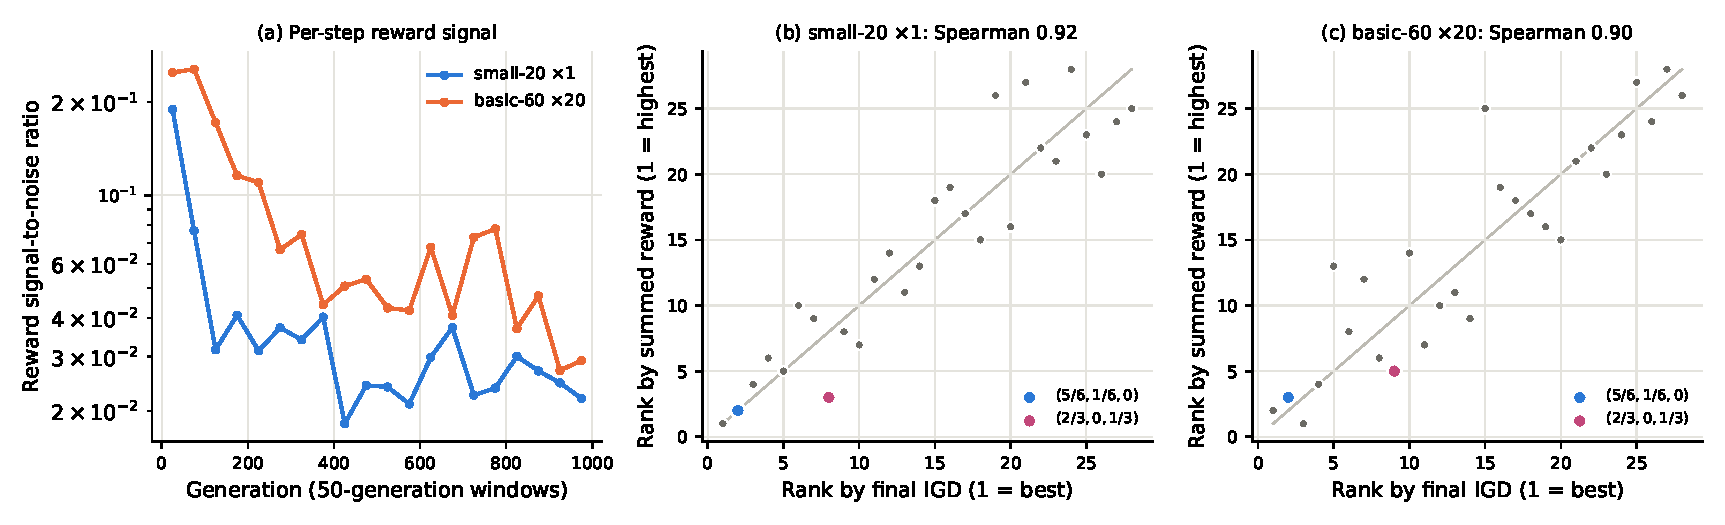
\includegraphics[width=\textwidth]{figures/d1_reward_audit.pdf}
\caption{Reward audit, each of the 28 actions held fixed for 1000 generations. (a) Signal-to-noise ratio of the
per-generation reward. (b, c) Rank of the summed reward against rank by final IGD.}
\label{fig:reward_audit}
\end{figure*}
